\subsubsection{Choix du solveur selon la composition des séquences}\label{sec:routage-composition}
Sur la matrice de surveillance, une esquisse peut indiquer une forte ressemblance même lorsque les deux séquences contiennent des nombres très différents de bases indéterminées. Les mots qui contiennent un tel symbole sont absents de l’esquisse, alors que l’alignement compte une substitution entre \texttt{N} et une base déterminée.

Soit \(n_i(a)\) le nombre d’occurrences du symbole \(a\) dans la séquence \(i\), symboles ambigus compris. En posant \(\Delta_a=n_i(a)-n_j(a)\) et \(x_+=\max(x,0)\), on obtient la borne
\[
   L_{ij}=\max\!\left(\sum_a (\Delta_a)_+,\ \sum_a (-\Delta_a)_+\right)
   \le d(i,j).
\]
Une édition élimine au plus un symbole en excès et comble au plus un symbole manquant. Pour les paires dont l’esquisse indique une forte ressemblance, le répartiteur choisit Edlib si \(L_{ij}\) atteint 5\,\% de la longueur de la séquence la plus longue. Les autres restent sur WFA2.

Sur les 64 génomes du SARS-CoV-2, les 2\,016 indices de Jaccard estimés vont de 0,531 à 1. Dans une première série de six blocs, le routage par mots seuls les envoie donc tous à WFA2. Il prend \(6{,}620\pm0{,}008\)\,s, contre \(2{,}448\pm0{,}006\)\,s pour Edlib seul sur les mêmes quatre cœurs Grace.

La figure~\ref{fig:routage-composition} compare les deux règles dans une seconde série de huit blocs. L’affectation par composition confie 610 paires à Edlib et 1\,406 à WFA2. Toutes restent sur CPU. Le calcul des esquisses et des affectations prend \(5{,}063\pm0{,}063\)\,ms. Les quatre politiques restituent les mêmes distances, qui servent ensuite à comparer les groupes de lignage.
\chart{comparison/routage_composition.png}{Temps moyen des 2\,016 alignements sur quatre cœurs Grace, après lecture du FASTA. Les traits indiquent l’écart-type et l’intervalle de Student à 95\,\% sur huit blocs. Les deux répartitions incluent le temps de choix du solveur.}{fig:routage-composition}{python/studies/hybrid_matrix.py}

Pour situer le travail sur CPU, LProf échantillonne le programme de routage sur quatre cœurs EPYC~9654 pendant une chauffe et six calculs de la matrice. La figure~\ref{fig:maqao-route} attribue 85,07\,\% des échantillons à la fonction de Myers d’Edlib et 10,97\,\% à l’extension des correspondances de WFA2. La construction des esquisses en reçoit 0,12\,\%. Dans une comparaison distincte sur un même exécutable, MAQAO~2025.1.4 et 2026.1.1 donnent les mêmes recommandations pour les 17 boucles et les 12 fonctions analysées par les deux versions de CQA. Deux fonctions de WFA2 reçoivent un diagnostic dans le seul profil de 2026.1.1. Le calcul des bornes du front représente 0,0173\,\% des échantillons et l’allocation des fronts 0,0189\,\%.
\begin{figure}[!htbp]\centering
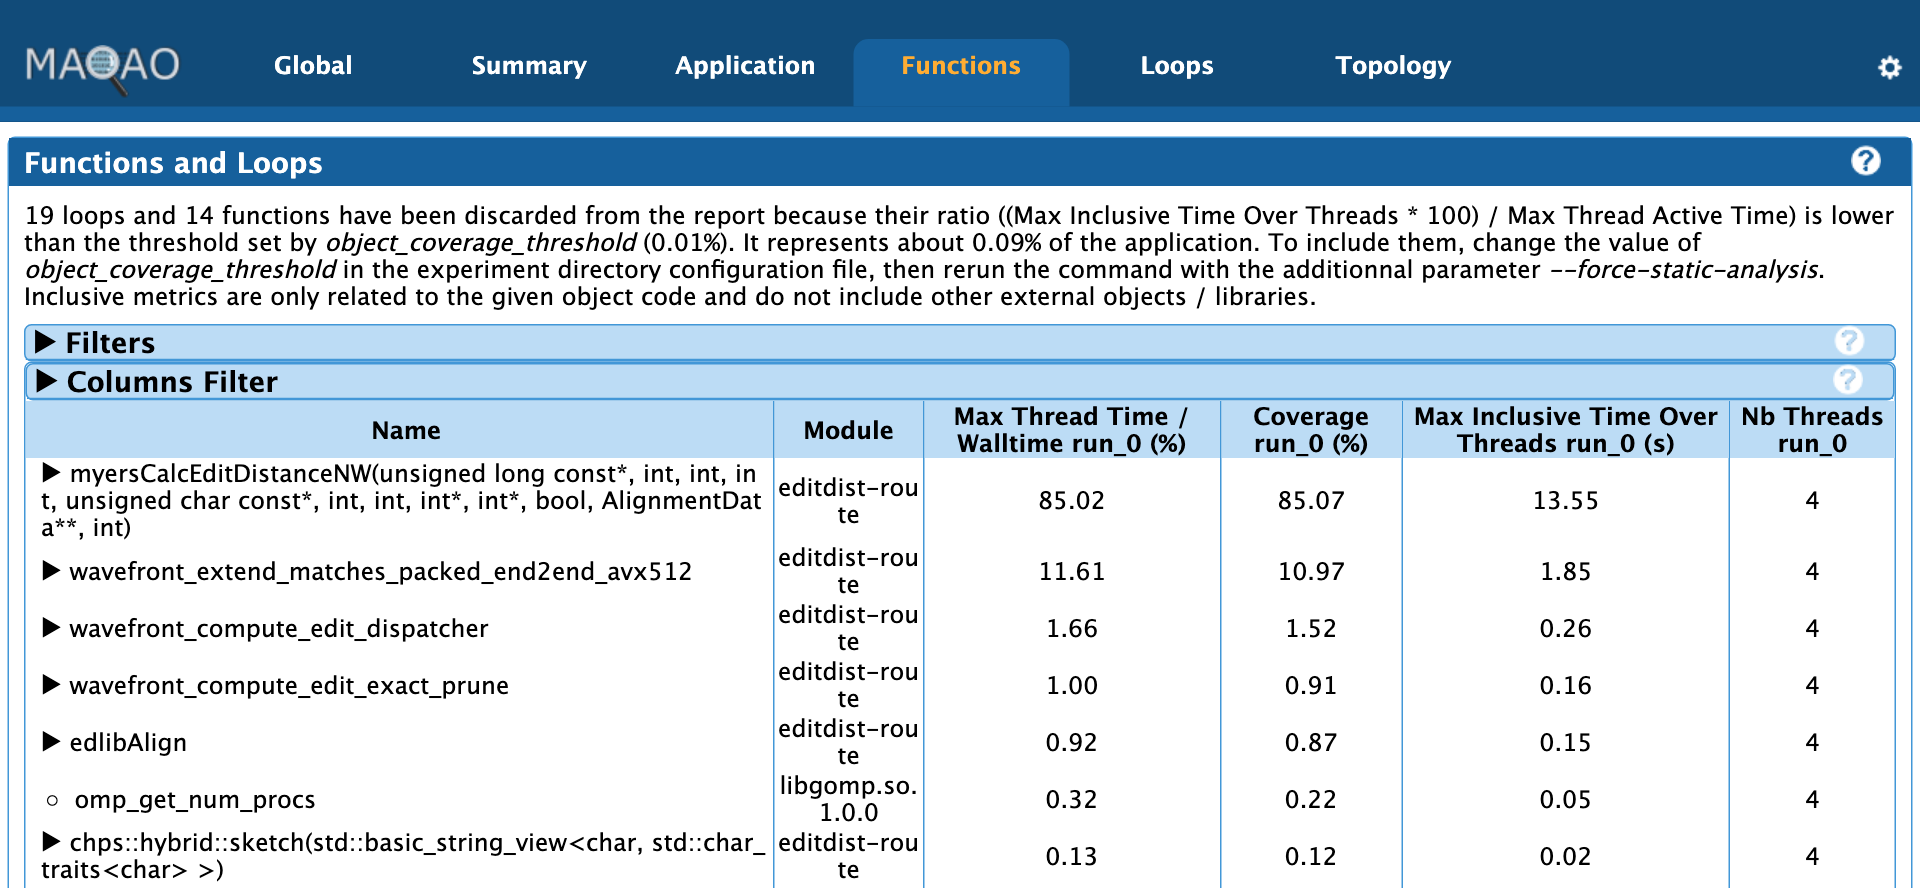
\includegraphics[width=.93\linewidth]{figures/maqao/fonctions-routage.png}
\sourcefig{bench/cpu/maqao/route.sbatch}\caption{Le profil des fonctions de MAQAO classe les routines pendant le calcul répété de la matrice de 2\,016 paires. La colonne \textit{Coverage} donne la part des échantillons de cycles.}\label{fig:maqao-route}
\end{figure}

\synthese{La règle de composition ramène le temps de \(2{,}433\pm0{,}016\)\,s avec Edlib seul à \(2{,}241\pm0{,}004\)\,s. Sur cette matrice, la réduction moyenne par bloc vaut 7,9\,\% (IC à 95\,\% de 7,4 à 8,4\,\%).}
